% common arguments
\newcommand{\coursenum}[0]{CSCI 0202}%
\newcommand{\coursetitletop}[0]{Computer}%
\newcommand{\coursetitlebottom}[0]{Architecture}%
\newcommand{\bordercolor}[0]{2827FF}%
\newcommand{\backgroundcolor}[0]{FFFFFF}%


\documentclass{standalone}
\usepackage{graphicx}
\usepackage{tikz}
\usepackage{xcolor}
\usepackage{inconsolata} % change to control font
\renewcommand*\familydefault{\ttdefault} 
\usepackage[T1]{fontenc}
\usetikzlibrary{backgrounds}

\begin{document}

\definecolor{border_color}{HTML}{\bordercolor}%
\definecolor{background_color}{HTML}{\backgroundcolor}%

\begin{tikzpicture}

  \newdimen\R
  \R=1in
  \fill [opacity=1,background_color]
  (30:\R)--(90:\R)--(150:\R)--(210:\R)--(270:\R)--(330:\R)--cycle;

  \node[]             at   (0.0, .1)     {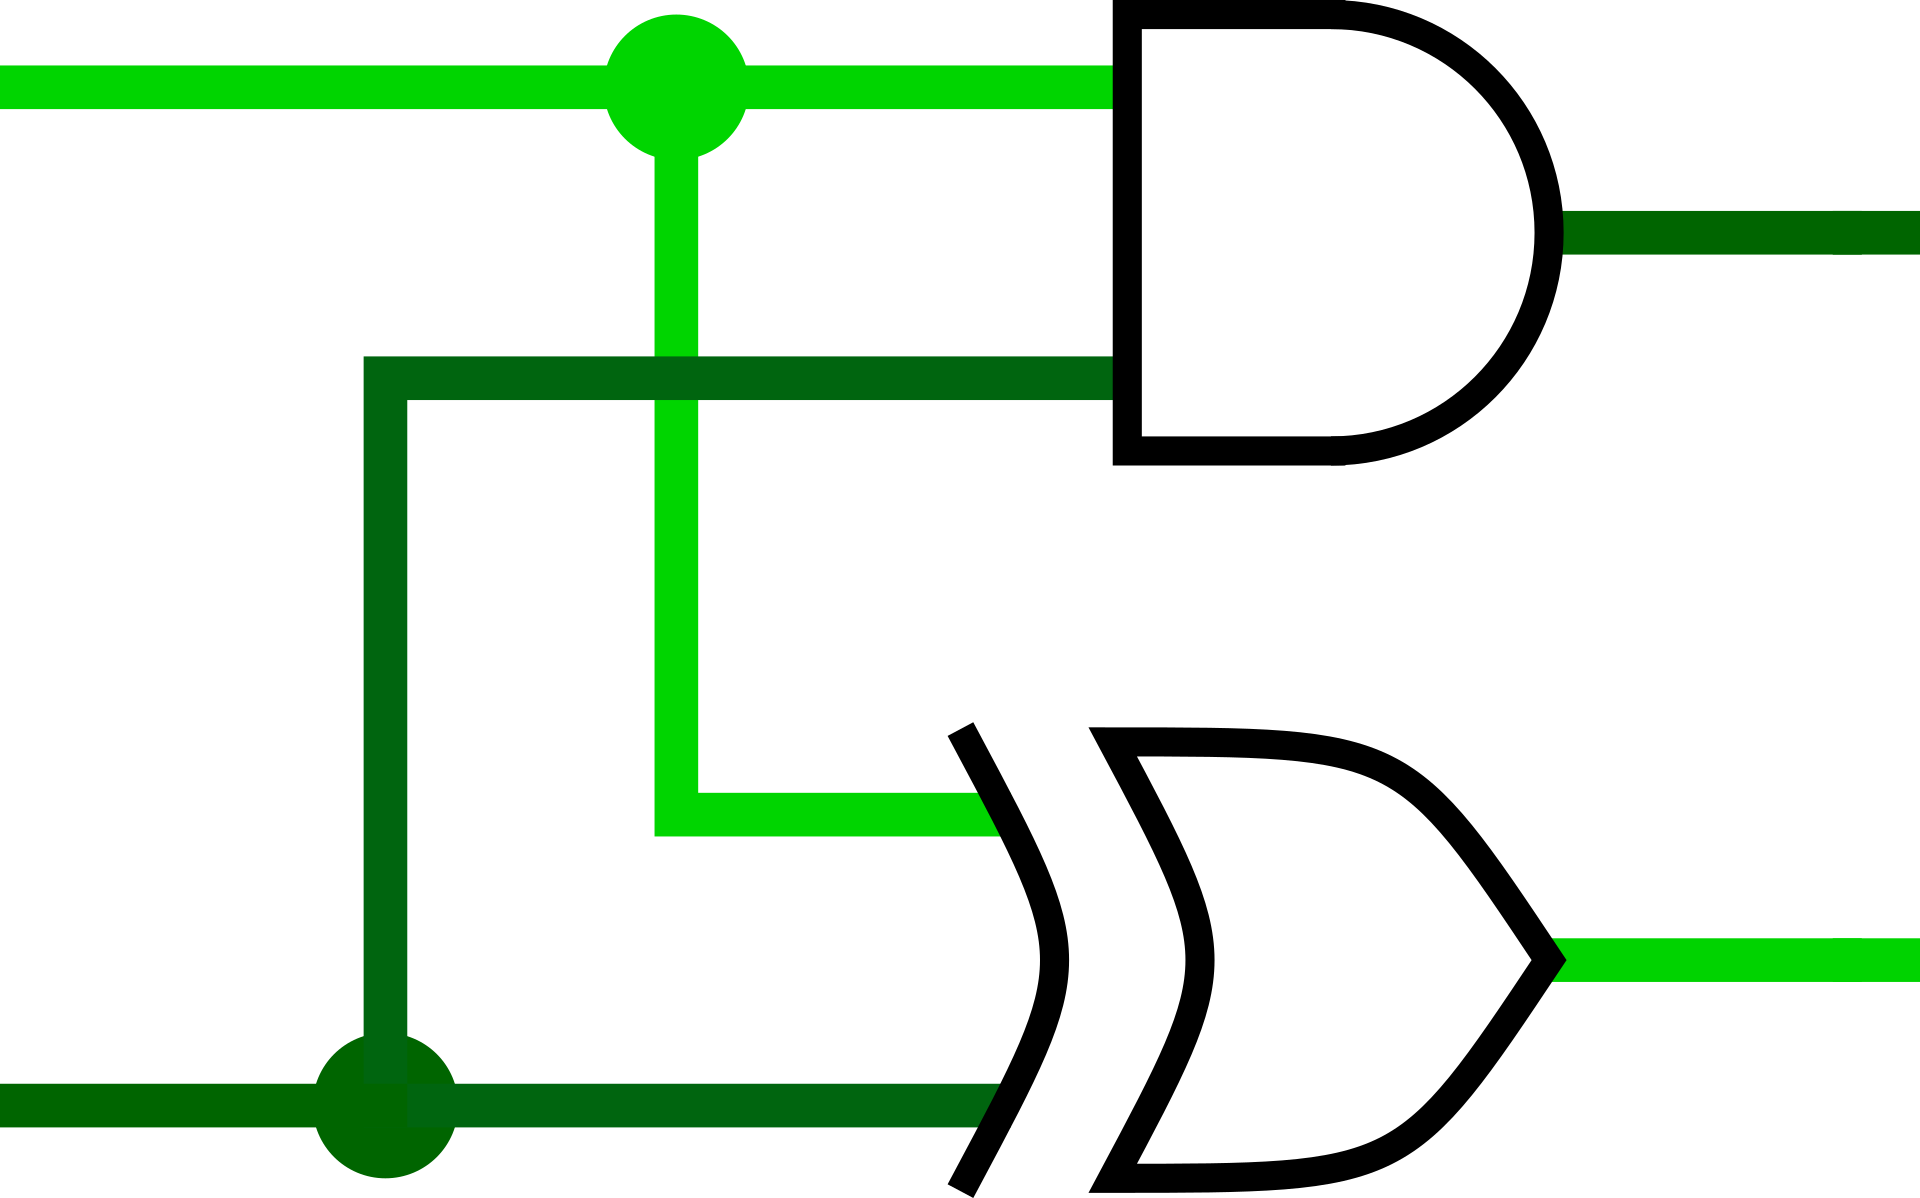
\includegraphics[height=0.6 in]{half-adder.png}};
  \node[align=center] at  (90:0.52in) {\Large \ttfamily \bfseries \coursenum};
  \node[align=center] at (270: 0.5 in) {\large \ttfamily \coursetitletop \\ \large \ttfamily \coursetitlebottom};
  
  \draw[rounded corners=0.3mm,line width=1.3mm,color=border_color]
    (30:\R)--(90:\R)--(150:\R)--(210:\R)--(270:\R)--(330:\R)--cycle;


  \end{tikzpicture}

\end{document}


